\section{Evaluation}
\label{sec:evaluation}
In order to evaluate the efficacy of our approach, we evaluated \sysname in both controlled and in-the-wild deployments.  

\subsection{Controlled Experiments} 
We evaluated \sysname's performance under controlled conditions in three phases to test different variables the system might encounter:

In \textbf{phase one} we tested \sysname on multiple doorways, with different characteristics---light levels, flooring, doorway heights and doorway widths.
For each test, we primarily evaluated \sysname's ability to detect someone passing through and determine the person's direction of movement.
We also tested the system's robustness to human variation, like height, clothing, and hair color by including a diverse group of subjects.
We tested on \numDoors different doorways with \numPeople people for a total of \numExp different doorway events (each person walked through multiple times per doorway).\footnote{This study was approved by our Institutional Review Board.}

In \textbf{phase two} we test the limits of the device, examining the factors that affect its accuracy, performance, and availability---including lighting conditions, walking speed, and short delays between doorway events.
We also tested a variety of events that may be falsely detected as doorway events.

In \textbf{phase three} we explore the energy harvesting ability and gather microbenchmarks of the energy consumption of the parts of the \sysname system.

\begin{table*}[t]
\footnotesize
	\begin{tabular}{@{}p{0.6in}p{0.5in}p{0.5in}p{0.45in}p{0.6in}p{0.3in}p{0.7in}p{0.7in}p{0.5in}@{}}
	\toprule
	\multirow{2}{*}{\textbf{Doorway \#}}	&	\multicolumn{2}{c}{\textbf{Light Intensity (lux)}} & \multicolumn{2}{c}{\textbf{Flooring}} & \multicolumn{1}{c}{\textbf{Enough}} & \multicolumn{1}{c}{\textbf{Total}} & \multicolumn{1}{c}{\textbf{Detection}} & \multicolumn{1}{c}{\textbf{Direction}} 		\\
	& Inside & Outside & Inside & Outside & \multicolumn{1}{c}{\textbf{Light?}} & \multicolumn{1}{c}{\textbf{Events \#}} & \multicolumn{1}{c}{\textbf{Accuracy(\%)}} & \multicolumn{1}{c}{\textbf{Accuracy(\%)}}\\\midrule
	1 & 86 & 96\textsuperscript{*} & Tile & Tile & Yes & 162 & 93.82 & 98.02 \\ %Lab Door
	2 & 86\textsuperscript{*} & 64 & Carpet & Tile & Yes & 63 & 90.48 & 78.94 \\ %224
	3 & 71 & 55 & Carpet & Tile & Yes & 106 & 100 & 98.11 \\	%Jacob's office
	4 & 96 & 111\textsuperscript{*} & Tile & Tile & Yes & 106 & 100 & 98.11 \\ %232
	5 & 55 & 55 & Tile & Tile & Yes & 112 & 99.1 & 94.59 \\ %hallway1
	6 & 55 & 71 & Tile & Tile & Yes & 102 & 100 & 96.08 \\\midrule %hallway2
	7 & 40 & 71 & Carpet & Tile & No & - & - & - \\ %226-1
	8 & 24 & 72 & Carpet & Tile & No & - & - & - \\ %226-2
	9 & 24 & 55 & Tile & Tile & No & - & - & - \\ %hallway-119
	\bottomrule
	\end{tabular}
	\caption{Evaluation results with 12 test subjects having variable heights, hair color, and clothing as described in \secref{sec:normal_operation}. We tested 9 different doorways, from which 6 had enough light to power \sysname. We ran multiple people through each of these 6 doorways, noting the detection accuracy and how many of the detected events had correct direction. These results show that an adequately-lit \sysname occupancy monitor can accurately detect doorway events and their directions.
	\vspace{1mm}
	\\\textsuperscript{*}Mixed Lighting --- Combined natural and artificial light
	\label{tab:detection}}

\end{table*}



\subsubsection{Methodology and Claims}
The following experiments address the goals defined in \secref{sec:system}.
We address system availability~(Goal~1) by demonstrating the low power draw of the system itself and the number of times it caught doorway events (and the number of doorway events missed) for each doorway test.
% the minimum light intensity at which \sysname can sustain operation and detect doorway events.
Further, we evaluated the accuracy in determining the direction~(Goal~2) by observing how often \sysname correctly determined walking direction.
We explored variable lighting conditions~(Goal~3) by testing the device under \numDoors different doorways with diverse lighting conditions, both typical and adverse.
We address human variation~(Goal~4) by evaluating different walking speeds and the effect of clothing and hair color/hair covering on detection patterns.
We claim that~(Goal~5), concerning form factor, is addressed by our prototype and slim mechanical design, described in \secref{sec:implementation}.

We also tested the limits of the device, by varying different factors to see when the device stops working and generating conditions that can confound the sensor.
These tests cannot hope to cover all possible deployment conditions, but they do give a broad sense of the capabilities and limitations of \sysname.

We gathered all electrical signal measurements, except where specified otherwise, using the Saleae Logic~16 logic analyzer\footnote{https://www.saleae.com} at a sampling rate of 5KS/s.
The analyzer's high impedance ADCs allow for unobtrusive signal monitoring.
This sampling rate is sufficient to detect the types of slow-varying doorway events that human activities produce.
We manually recorded the direction of each doorway event as ground truth to verify the accuracy of \sysname in event detection, then compared the ground truth results with the results measured by the logic analyzer.
We measured light intensity levels using a TSL2561 Light-to-digital converter,\footnote{https://cdn-shop.adafruit.com/datasheets/TSL2561.pdf}
aligned to the same angle as the solar panels in both directions to get accurate light intensities falling on the panels.

Finally, we note that it is difficult to fairly compare the performance of different occupancy-monitoring systems except in their accuracy. For example, CeilingSee~\cite{yang2017ceilingsee} uses 16 devices to instrument a room, while \sysname and SonicDoor~\cite{sonicdoor-buildsys2017} place one device in the doorway, and AURES~\cite{shih2016aures} places a single device in the middle of a room. 
For this reason, we investigate the accuracy of \sysname against our manually gathered ground truth (visually verifying a person entering or exiting the room) instead of comparing to another occupancy-detection system.

%%only if time allows:
%%%passing vs. normal entering and exiting of the room
%%%what multiple people entering in close succession looks like to the system and can the system tell the difference between the systems.

%Notes on current testing plan environment:
%tile floor, semi reflective
%door open
%lights on on both sides of the door
%16 solar panels that are alternatively tilted by 10 degrees in either direction (8 panels on each side)
%walking at normal speed through the center of the doorway

%In order to test how well \sysname fares in terms of the availability goal, we tried turning down the light levels till \sysname stopped sustaining operation. Our aim in performing this experiment is to find a threshold above which \sysname sustains operation and is available for detecting ephemeral doorway events as they occur.
%We found that \sysname stops sustaining operation below XXYYZZ lux. This is an acceptable threshold as the average light levels in office environments will be greater than or equal to \SI{70}{\lux}. Even when the light levels fall significantly lower till \SI{40}{\lux}, we are able to detect events but it does affect our direction detection, as outlined in the next section.


\subsubsection{Normal Operation}
\label{sec:normal_operation}

In order to evaluate how well our approach detects doorway events, we tested \sysname across multiple different doorways with a diverse group of subjects.
In these tests, we focused on detecting doorway events caused by a person walking \textit{under} the doorway and accurately determining the direction of the person's movement.

\noindpar{Experiment Overview:}
We tested twelve~(12) different participants, with different physical characteristics---heights ranging from 5'4'' to 6'4'' and hair color ranging from blond to brown and black.
Our test group included a wide range of clothing colors (light and dark) and a variety of head coverings.


For this experiment, we affixed the \sysname prototype to the top of \numDoors different doorways.
\tabref{tab:detection} describes the doorways, including details like light intensity levels and flooring type.
For each doorway, we maintained test subject diversity, in order to characterize \sysname's performance, independent of the characteristics of individual subjects.
For doorways with doors, the door remained open throughout the experiments.
%This was done since
Each participant walked in and out of the room five times in each direction.

\noindpar{Results:}
The results of this experiment, including 651 individual doorway events, are shown in \tabref{tab:detection}.
Each \textit{event} consists of one person walking through one doorway one time.
\sysname successfully detected doorway events and the direction people were traveling through the doorway, detecting a total of \numDet events out of \numExp, giving an overall detection accuracy of \SysAccuracy.
Furthermore, it determined the walking direction correctly for a total of \numDir events, which is \dirAccuracy of the total events detected.
\sysname's performance was consistent across all test subjects, independent of human variations like height, hair color, and clothing.



\subsubsection{Factors affecting \sysname's operation}
\label{sec:confounding}

%\noindpar{Experiment Goals:}
In addition to testing ``normal'' walk through conditions, in this section we examine factors that affect \sysname's performance as an occupancy-monitoring sensor.
It would be impossible to exhaustively study all possible variations, but we are able to explore how \sysname reacts to a variety of conditions and behaviors that it will encounter in actual deployments.
Specifically, we explored the following factors:


\paragraph{Light intensity:}
We tested \sysname on a variety of doorways with varying lighting conditions, with results listed in \tabref{tab:detection}. 
Since \sysname's solar panels are sensitive to visible light and the IR spectrum, we used a TSL2561 sensor to measure both mixed signal (visible and IR) data along with purely IR data, and outputs the combined illumination value in lux.
As shown in \tabref{tab:detection}, our current prototype is fully functional on doorways with light levels above at least 55~lux on both sides.
An average room/hallway in an office-style setting has light levels around 70~lux, which is sufficient to power the \sysname sensor.
It is worth noting that we can customize \sysname for exceptionally dark doorways either by increasing the number of solar panels without changing the working of the system itself, or by employing input booster circuits like the ones used in CleanCut~\cite{colin2018cleancut}.

\paragraph{Walking Speed:}
\sysname detects people walking under doorways based on the changes they induce in the system's harvested energy supply.
This means that if a person walks slowly enough, their movement should become imperceptible to the system.
In order to evaluate this limit, we asked test subjects to walk under the sensor at different speeds.
We used a metronome to which the subjects could match their steps in order to achieve a consistent even speed.
With extremely slow walking (slower than 1~ft/s), we did observe decreased accuracies.
\sysname occasionally detected a slow-moving doorway event as two events.
No test subjects have yet been able to walk slowly enough to avoid detection entirely.
We don't consider this to be a problem for \sysname, since in practice, people don't often move at such slow speeds.

\paragraph{Door Width and Height:}
All doors except door \#4 (in \tabref{tab:detection}) were 80 inches tall, door \#4 was 87 inches tall. 
All doors except door \#6 were 34.5 inches wide, while \#6 was 58.5 inches wide.
A typical interior doorway is 32 inches by 80 inches.
In our experiments, the door width and height had no significant effect on the accuracy, however, we only tested when a single person went through a wide door, and we did not control for participants walking through the middle or side of the door (they were asked to walk naturally).


\begin{figure*}[t]
    \centering
    \begin{subfigure}[t]{0.38\textwidth}
        \centering
        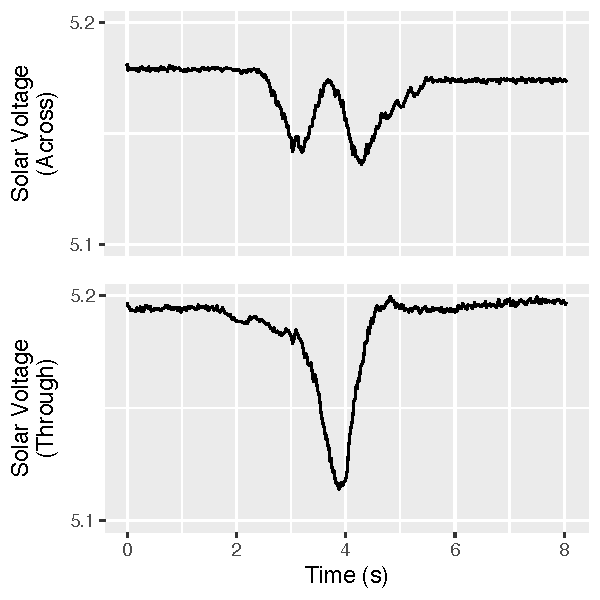
\includegraphics[width=\columnwidth]{figs/spotlight.pdf}
        \caption{These traces show the solar panel output in the presence of the ``Spotlight'' effect. The top figure shows the response when someone walks \textit{across} the ``Spotlight'', while the bottom one shows the response when someone walks \textit{through} the door.}
        \label{fig:spotlight}
    \end{subfigure}%
    %
    \hspace{30pt}
    \begin{subfigure}[t]{0.38\textwidth}
        \centering
        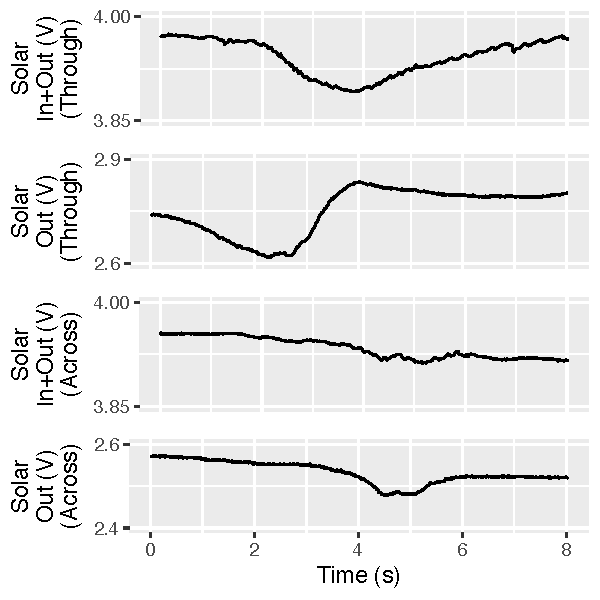
\includegraphics[width=\columnwidth]{figs/acrossAndLinger.pdf}
        \caption{ This figure compares a person walking \textit{through} the doorway (top two traces) versus walking \textit{across or by} the doorway on the outside. There is a clear delay between the two solar panel channels when someone walks through, whereas the change is reflected simultaneously when someone walks by.}
        \label{fig:across}
    \end{subfigure}
    \caption{Factors affecting \sysname operation. \label{fig:confounds}}
\end{figure*}


\paragraph{Multiple people:}
\secref{sec:normal_operation} showed the ability of \sysname to detect individual people walking through.
A practical consideration would be to consider the performance of \sysname when multiple people walk through.

In order to evaluate this, we tested two subjects walking through doorway \#1 with varying time delay between them.
This gave us control over the time separation between two events, and allowed us to examine how closely can two people walk in without being detected as one, quite large person.
We discovered that as long as two people have at least \minSeparation between them, \sysname can accurately distinguish between them.
This limitation is introduced due to the time required by the solar panels to reset or stabilize before the next event can occur.
A subsequent logical conclusion is that if two people walk side-by-side, \ie with zero separation between them, the current setup of the system is unable to detect them as two events.

\paragraph{The ``Spotlight'' effect:}
A very interesting consequence of light-based detection is what we affectionately call the \textit{spotlight effect}.
This effect appears in the presence of a very focused source of light that dominates the illumination around the doorway, such as a spotlight or a west-facing window in late evening when the sun blazes directly through.
When someone walks across such a focused light source, even if it's far from the doorway, it is detected falsely by \sysname as someone walking through.
This happens because \sysname detects people based on a decrease in the harvested energy, which also occurs when somenone momentarily blocks the focused source of light.
Interestingly, we can see from \figref{fig:spotlight} that the raw output of the solar panels look sufficiently different for someone walking \textit{across} the focused source as compared to when someone walks \textit{through} the doorway in presence of a focused source.
At present, \sysname is equipped to detect events with good accuracy.
With further signal processing, the difference between these events can be extracted so that such events will not cause false triggers.


\paragraph{Detection Range/Walking across, not through:}
\label{subsubsec:range}
Considering that \sysname uses the blocking of light to detect a person, there will be an influence radius inside which a person starts affecting the harvested energy of the sensor.
If someone walks by either side of a doorway monitored by the \sysname sensor and are within the influence radius of the sensor, they will affect the sensor readings.
We ran an experiment to determine this radius of influence where the subject was directed to walk by on either side of the doorway at increasing distances from the sensor.
We started with a distance of 1 foot and went up to 5 feet, in increments of 1 foot.
For each distance, we asked the subject to walk by multiple times and recorded how many false triggers were detected.
Our findings are presented in \figref{fig:across}.
We have observed that for distances greater than 3 feet away from the doorway, there is a negligible chance of triggering false events.

It is interesting to note from \figref{fig:across} that there is a distinguishable difference between this event as compared to someone walking through the doorway.
Since they are walking only on one side of the doorway, their effect on both channels is not delayed by the angling of the solar panels, as is the case with walking through.
As with the ``Spotlight'' effect, we should be able to extract this difference with further signal processing and learning and we attempted a stab at addressing this confounding condition further in the uncontrolled experiments that will be discussed later.  \fxnote{[This needs some serious rewording for the fact that we do try to handle this in the uncontrolled experiments.-NT]}

\paragraph{Lingering in the doorway:}
Another situation that causes false triggers is when a person comes up to the doorway, but simply pokes their head in.
Upon evaluation, we discovered that as long as the person is poking their head in the doorway, the solar panel output remains at a lower level, and when they exit, it rises back again.
Although the current system implementation isn't equipped to differentiate between someone passing through and someone lingering in doorway, there is a clear difference in the raw waveform outputted by the solar panel.
This case is similar to \secref{subsubsec:range} in terms of being distinguishable from a person walking through and with some careful, direct signal processing it is definitely possible to differentiate between the actual and the confounding case.

\subsubsection{Microbenchmarks}
\label{sec:microbenchmarks}
The more effective \sysname is at maintaining a low-power state when idling, the more available \sysname is for detecting doorway events and monitoring occupancy.
The energy requirements for detection and active computation must be kept low as well.
Unlike intermittent computing systems, \sysname must intentionally avoid power failures.
We measured the current draw of our \sysname prototype while it was mounted on doorway \#1.
The idle draw of the system was \SI{18}{\micro\ampere}, showing that \sysname can survive in a doorway with minimal light and energy harvesting.
We gathered other benchmarks of system energy performance in each mode of operation \sysname enters; the results of our experiments are shown in \tabref{tab:microbenchmarks}. These measurements were made after the MIC841 hysteresis chip, so the actual power and energy is slightly higher (by \SI{1.5}{\micro\ampere} according to the datasheet).


% Idle Current: 7-11uA, MCU not active
% Timer / ISR handling, single detector, no event : 190-230us, MCU active
% Doorway Event, MCU active, compute time: 7.2ms
%
% Peak current for active: 500uA
% Avg current for active: 220uA
% 2.8V
\begin{table*}[t]
\footnotesize
\begin{tabular}{@{}p{1.4in}lllc@{}}
\toprule
\textbf{State}          & \multicolumn{1}{r}{\textbf{Avg. Power}} & \multicolumn{1}{r}{\textbf{Peak Power}} & \multicolumn{1}{r}{\textbf{Energy Cost}} & \multicolumn{1}{r}{\textbf{MCU Active}} \\ \midrule
\textit{Waiting (Deep sleep)}       	& \SI{7}{\micro\ampere}	&  \SI{11}{\micro\ampere}	& - & \textcolor{magenta}{\xmark} \\
\textit{Maintenance Actions} & \SI{220}{\micro\ampere}	& \SI{500}{\micro\ampere}	& \SI{140}{\nano\joule}	 & \textcolor{green}{\cmark} \\
\textit{Doorway Event Handler} & \SI{220}{\micro\ampere}	& \SI{500}{\micro\ampere}	&  \SI{4424}{\nano\joule}     & \textcolor{green}{\cmark} \\ \midrule
\end{tabular}
\caption{Microbenchmarks for \sysname energy consumption.}
\label{tab:microbenchmarks}
\end{table*}


\tabref{tab:microbenchmarks} shows a low quiescent current where the MCU is asleep (the Idle state) of \SI{7}{\micro\ampere} on average. Maintenance events (from timer firing or single detectors firing from noise or people passing by the doorway but not walking through) only require \SI{140}{\nano\joule} to handle in active mode with the MCU running.
The most expensive compute operation is when the detectors fire and the MCU must compute the direction and store the results to non-volatile memory: FRAM. This costs \SI{4424}{\nano\joule}.
Overall the energy consumption of the system is low, but could be further improved with careful tuning of resistance values, sleep states, and the analog circuitry.

\begin{table*}[t]
\footnotesize
	\begin{tabular}{@{}p{0.65in}>{\centering\arraybackslash}p{0.4in}>{\centering\arraybackslash}p{0.4in}p{0.4in}p{0.5in}p{0.6in}p{0.55in}p{0.55in}p{0.55in}p{0.55in}p{0.5in}@{}}
	\toprule
	\multirow{2}{*}{\textbf{Doorway}}	&	\multicolumn{2}{c}{\textbf{Dimensions (in)}} & \multirow{2}{*}{\textbf{Light}} & \textbf{Total} & \textbf{Gnd Truth} & \textbf{Detected} & \textbf{Accounted} & \textbf{Extra} & \textbf{Missed} & \textbf{Recall}		\\
	& Height & Width &  &  \textbf{Days} & \textbf{Events} & \textbf{Events} & \textbf{Events} & \textbf{Events} & \textbf{Events}\\\midrule
	Lab & 79.5" & 34.5" & Mixed & 8 & 445 & 735 & 354 & 388 & 91 & 74.02\% \\ %Lab Door
	Hallway & 76.0" & 93.0" & Indoor & 4 & 753 & 660 & 731 & 109 & 22 & 87.66\% \\ %hallway
	Classroom & 87.0" & 35.0" & Mixed &  9 & 213 & 300 & 167 & 107 & 46 & 68.84\% \\	%232
   
	\bottomrule
	\end{tabular}
	\caption{In-the-Wild evaluation results for three different locations, from data collected over multiple days for each location. \sysname effectively detected doorway events and other activities around the sensor, while troublesome cases like people lingering under/around the sensor can produce additional event information for a single event. 
	\vspace{1mm}
	\label{tab:ITWresults}}

\end{table*}



\subsection{\sysnames in the Wild}
\begin{figure}[t]
\centering
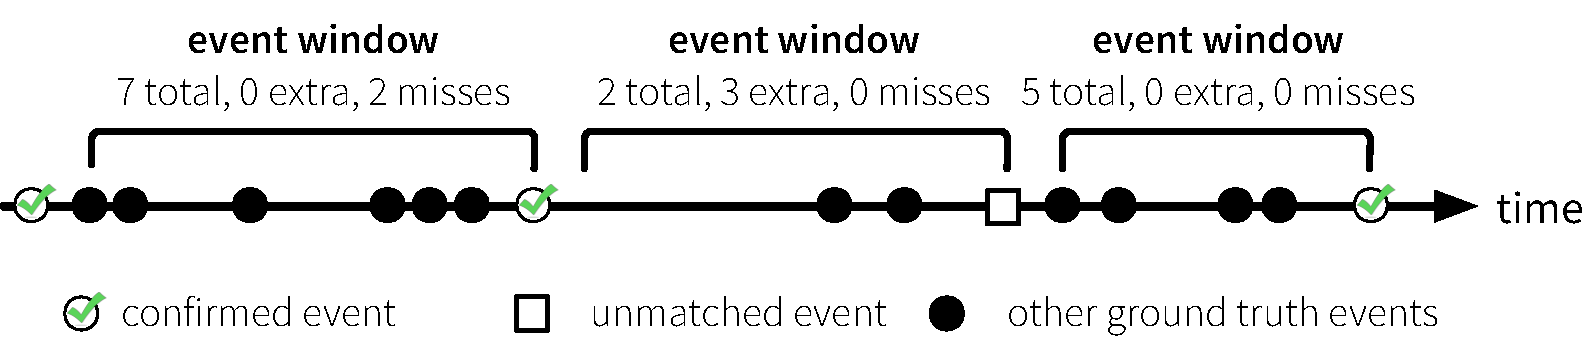
\includegraphics[width=1.0\columnwidth]{figs/timeline.pdf}
\caption{ The ground truth event timeline of our in-the-wild deployment and how it is divided up into windows based on the anchor packets.  This example provides a high level view of how we compute the event statistics within a window.  \label{fig:eventtimeline}}
\end{figure}
%setup

We conducted an extensive in-the-wild deployment of multiple \sysname units.
The controlled experiments helped us understand some of the major limits of the system, but we also wanted to see how it fared in an in-the-wild deployment.  
For a real-life application evaluation, we installed \sysname on two doorways and a hallway, gathering \ITWdays collectively of all-day occupancy data with visual (camera based) confirmation of ground truth. 

\subsubsection{In-Wild Experimental Setup.}
We chose locations---a lab door, a classroom door, and a hallway---that differ in light levels, width, and height, while providing a range of lighting and behavioral conditions. 
For example, the classroom door encounters multiple confounding cases like lingering and crowds passing under the doorway, while the lab is affected by lingering and spotlights.
Dimensions for these locations are reported in \tabref{tab:ITWresults}.  %The lab doorway is 34.5" x 79.5" and the light level is 86 lux inside the room and 91 lux outside of the room. The classroom doorway is 35" x 87" and the light level is 91 lux inside the room and 100 lux out of the room. The hallway is 76" x 93" and the light level on one side of \sysname is 94 lux and 89 lux on the other side. 
All doorways in this deployment have tile flooring and are typically well enough lit to transmit a packet once for every five detected doorway events. 
Besides \sysname devices we deployed two continuously powered basestations to collect the transmitted data from the batteryless \sysname devices.
Each basestation is an Internet-connected Raspberry Pi with a CC1101 radio that receives packets and logs them to a SQL database stored in the FLASH memory of the Pi. This data is easily retrieved for later classification of events.  

At each instrumented doorway we also place a motion activated camera that collects ground truth information by recording the actual doorway events. 
We manually labeled all recorded events by watching the videos and annotating and storing the time and a description of each event---\textit{in, out, pass-by}, as well as confounding cases like lingering and multiple people passing in or out.

We compare this source of ground truth against the events \sysname detects.
\sysname attempts to send a message to the basestation only after gathering a total of five detected events (sometimes more, since there must be enough energy to send and events may be detected while waiting for energy to send).
\sysname summarizes the events, their classifications, computes and stores a CRC over the values to protect against packet corruption and sends the summary of the collection to a nearby basestation where it will be logged for analysis. 
Each packet also encodes a small legacy of the information received in the last two packets to guard against packet loss. 

\sysname does not currently report time information, so the time the basestation receives a packet is used as a reference to match windows of events to the ground truth data.
Since \sysname reports summaries after every five events, the basestation's receive time is closely correlated to the last event in the summary.
We use these times to match likely event windows in the ground truth with received packets sent by the \sysname sensors.

%Looking at high level detection of events
\subsubsection{Data Collection and Analysis Method.}
Each packet (encodes a summary of at least 5 events) received at the basestation is matched to a likely ground truth event as long as the time between the two is less than 30 seconds.  
This helps account for human error in labeling event times as it is not always clear exactly when someone started affecting the sensor from video data.
If two events match a packet, the one closest (in time) is chosen and mapped to the 5th event associated with this packet.
Packets that map to a ground truth event are considered \textit{confirmed packets}.
All other packets that could not be mapped to an event (within 30s), are still valid packets that represent five events that \sysname detected and must be considered. 
We insert these packets into the event sequence and mark them as \textit{false positive} packets.
The false positive packets may still contain valid data associated with the ground truth.
The fifth event that generated the packet may have just been missed in the ground truth. 
These confirmed and false positive markers divide up the ground truth data into probable event windows in order to make a meaningful comparison with the packet summaries.
We then gather statistics on the number of probable events associated with each packet. 
Confirmed packets are included in the associated window counts, however, false positive packets, while still providing a meaningful anchor for the probable event window, did not have an event closely associated enough to add to the probable event window counts.  

We reason about the number of events that \sysname actually detects in these ground-truth based probable event windows by drawing on two characteristics of the system design. 
One, each packet encodes five events, and two, every packet will have a different packet id number, one greater than the last packet.
Using this knowledge, we can figure out which packets, if any, we missed (what packet id numbers were absent on the basestation?) and how well \sysname \textit{detected events}, even if it may have classified events incorrectly.
When all the ground-truth events in the event window were explained by the number of events in the anchor packet and missed packets, we considered the window to be accounted for. 
When they are not, we know that either events were recorded (on video) but not detected by \sysname, denoted as \emph{misses}, or \sysname detected more events than were reported in the ground-truth data, which we called extras. 
\figref{fig:eventtimeline} shows a high level example of the how ground truth events are divided by the anchor packet time in order to calculate extras and misses. 
These values are aggregated over all probable event windows in the ground truth data.

The results, shown in \tabref{tab:ITWresults}, are mixed.  
\sysname did a decent job of detecting when activity was taking place near the sensor, with few missed events.
After inspecting the data, nearly all misses appear to come from three situations: (1)~a person passed by the doorway, far from \sysname but still visible to the camera; (2)~multiple people passed by the door in close succession, seen as multiple events by the ground truth labelers, but only a single event by \sysname;
(3)~packets were lost due to \sysname power failures and sequences of dropped packets. 
Extra events were far higher than missed events in our data, primarily due to long and slow events---particularly common around the lab and classroom---many of which lasted minutes, were labeled as a single ground truth event but misclassified by \sysname as many events (mostly passbys).
\sysname clearly has room for improvement when classifying confounding cases like lingering and other long events and high-traffic situations; however, even in these problematic cases, \sysname serves as an effective activity sensor. \fxnote{I want to say somewhere in here that other PIR or Ultrasound-based sensors are going to have a hard time with this, too. -JMS}

%for recall event classification results
\subsubsection{Results.}
After evaluating \sysname event detection in general, we processed the data in a different way to reason about the system's classification accuracy. 
\sysname's design makes it difficult to reason about true negative events. When there was no activity, no videos were recorded and \sysname did not report events.
This is intended behavior, but without discrete negative cases statistical measures are meaningless.
Instead, we focus on the true positive rate, or Recall, as reported in \tabref{tab:ITWresults}.   

We process the data slightly differently, in order to assess how the system classified events.
We map all received packets to their closest matched ground truth event.
As before, this marks the end of the collection of ground truth events that likely contributed to the creation of the associated packet.
The matching ground truth window ends at the packet's receive time and includes up to the prior 5 events as long as they are not included in another packet's likely matched window. 
This means that some of our event windows contain fewer than five events, usually due to a linger event that is seen by \sysname as multiple events. 
We compare these likely-matched event windows to number of ins, outs, and passbys reported in the received packets and compute the true positive rate (recall).
Our classification accuracy ranged from 69-87\% depending on the location, with highest accuracy in the hallway where people tended to walk more and linger less.  


%\subsubsection{Discussion of In-Wild Results.}
%These results are impacted by people lingering by doorways, entering or exiting in crowds, making abrupt changes in direction under the sensor, and by individuals changing out cameras to collect ground truth or preforming basic system maintenance.  The matched windows to draw our comparison was impacted by sporadic camera malfunctions which limited available ground truth, collection over spring break which dampened overall user activity for several days, and a school wide power-outage for system maintenance which impacted the available light to the sensors as well as the power for the basestations to collect data and log them to the SQL database.


%\fxnote{[ I created  confusion matrix using R based on the collected data, but that data needs some cleaning like i+o, (i+)o in the %detected direction-AA]}
%section:  System Accuracy
	%just walking through
		%-just using interrupts
		%-just detection circuits
		%hw detection only vs sw enhancements
	%detecting direction
		%-just using interrupts
		%-just detection circuits
		%hw detection only vs sw enhancements
%if we get to sw at all





%section:  extreme cases (how low can we make lighting and system still work)?
